\section{Solution Design and Implementation}
\label{sec:parallelization}

\subsection{Parallelization With OpenMPI}
To harness the speedups offered by parallel computing, we used the OpenMPI\footnote{\texttt{\url{https://www.open-mpi.org}}} library.
The first step was to choose which part of the program to parallelize.
The recursive part was the immediate candidate.
We decided to read all the input points in the first process, \textnumero~0, then distribute them uniformly to all available processes, including \textnumero~0.

The next step was deciding how to communicate amongst the processes to combine the results effectively.
We decided to adopt the scheme illustrated in
\Cref{fig:albero_bell_albero}.
Every process, numbered $p$, iteratively communicates its result to another destination process, if it did not already do so.
Having $i$ as the iteration number and starting from $i$ equal to zero, the number of the destination process is equal to $p-2^i$.
Process \textnumero~0 is the only exception: it always receives.

\begin{figure}[ht]
    % \resizebox{\columnwidth}{!}{
    %     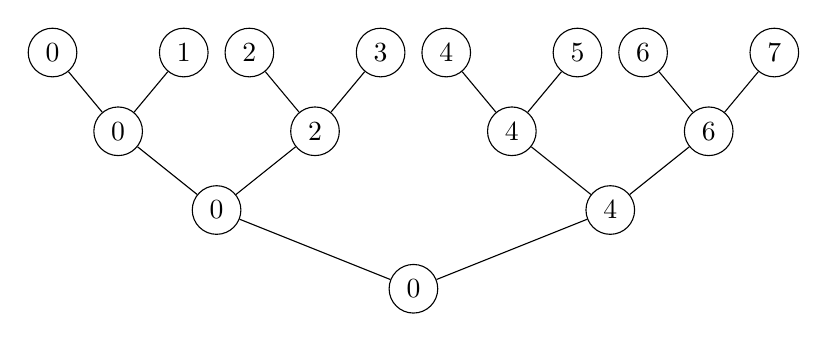
\begin{tikzpicture}[
        grow'=up,
        every node={
                style={
                        draw,align=center
                    }
            },
        level distance=1cm,
        level/.style={sibling distance=5cm/#1}
    ]
    \tikzset  {
        treenode/.style = {circle, draw=black, align=center, minimum size=0.5cm},
    }
    \node [treenode] {0}
    child {
            node [treenode] {0}
            child
                {
                    node [treenode] {0}
                    child {
                            node [treenode] {0}
                        }
                    child {
                            node [treenode] {1}
                        }
                }
            child
                {
                    node [treenode] {2}
                    child {
                            node [treenode] {2}
                        }
                    child {
                            node [treenode] {3}
                        }
                }
        }
    child {
            node [treenode] {4}
            child
                {
                    node [treenode] {4}
                    child {
                            node [treenode] {4}
                        }
                    child {
                            node [treenode] {5}
                        }
                }
            child
                {
                    node [treenode] {6}
                    child {
                            node [treenode] {6}
                        }
                    child {
                            node [treenode] {7}
                        }
                }
        }
    ;
\end{tikzpicture}

    % }
    \centering
    \includesvg{../assets/graphics/tree_merge.svg}
    \caption{Illustration of the process communication scheme with 8 processes.}
    \label{fig:albero_bell_albero}
\end{figure}

With the communication scheme defined, we proceeded starting its implementation with the OpenMPI library.
Given our communication requirements, we added two custom MPI datatypes: \verb|mpi_point_type| to represent a point and \verb|mpi_pair_of_points_type|
to represent a pair of points.

Next, we decided which MPI calls to use.
Given that process \textnumero~0 is the one that reads the file initially, and therefore the only one that knows the total number of points, the natural choice to distribute such number to all the other processes was a broadcast with \verb|MPI_Bcast|.
After that, each process allocates the memory it will need to store its share of the points, which is communicated by process \textnumero~0 through an \verb|MPI_Scatterv|.
Each process then sorts its points individually using the serial implementation.

After a process computed its closest pair, it sends the best closest pair candidate to the receiving process through a call to \verb|MPI_Send|. It then computes the bands of points to send to the receiving process, according to the smallest distance it found. Once it has computed the bands, it first sends -through an \verb|MPI_Send|- a pair of integers to the receiving process representing, respectively, the lenght of the left and the right band. It then transmits, always through an \verb|MPI_Send|, the points, in a single array where the left points are followed by the right points.

\noindent
This arrangement allows us to have three MPI send operations in total for each process `merge' step\footnote{Further optimizations are proposed in \Cref{subsec:future_works}}.

\noindent
Finally, each receiving process will look in the band for a closest pair than the one computed before.
The whole cycle will be repeated until the process \textnumero~0 will be the only one remaining.

\subsection{CI/CD Setup}

Writing code is undoubtedly a core part of the software development process, yet as the complexity of the project increased in time, good software engineering practices became more and more important in helping to keep the growth of the codebase under control.
%As in security, we like to remove things that can fail from the loop, and these are humans. Sorry humans.

In particular, we decided to set up a version control system with git\footnote{\texttt{\url{https://git-scm.com}}} from the get-go, hosting on GitHub. After that, we added Continuous Integration through the use of GitHub Actions and Google Test framework\footnote{\texttt{\url{https://google.github.io/googletest}}}. The CI pipeline is minimal, but effective in preventing regressions: every time a push - or a pull request- is made, the code is compiled with the same compiler, \verb|mpicc|, that is used on the cluster and tests are run. Our actual tests perform a small run of the algorithm in order to check if it outputs the expected result.

If everything until now went well, the GitHub Action proceeds in doing another small test run on the cluster. In order to do so, it copies the source code to the cluster, compiles it and submits a job with a medium sized dataset -1M \mbox{points-,} asking for 2 CPUs and 2 chunks, with a time limit of 5 minutes. When the job completes -or fails-, we are notified through a Telegram bot, which also sends us the output files.
Each run is assigned a petname \cite{ferdous2009petnames} and a UNIX timestamp for easy identification and is stored in a dedicated subdirectory, so everything is retained if we need to inspect it later on.

Since we are running on a shared cluster, our scripts include automatic checks -and alerts- to ensure we are not using more storage than we are allowed to use.

\vspace{0.2cm}

Next, we automated the execution of the benchmarking tests.
These are managed by a pipeline that is triggered when we create a new tag in the repository.
The benchmark pipeline executes the same tests as the other pipeline, with the only difference that instead of creating a single job, it sequentially submits to the cluster -one at a time- the combinations of inputs and job parameters we want to test -namely: number of chunks, number of CPUs, and placing strategy-. The script checks the status of the submitted job every 10 seconds. Once the job is finished, it collects its results and adds them to a new row in a Google spreadsheet
\footnote{Link in \Cref{link:spreadsheet}}.
The benchmarking script executes everything four times, and notifies us on Telegram as it progresses and when it finishes.
As with the CI, every benchmark run in the cluster is neatly organized in its own subdirectory, with timestamp and petname.

Since the datasets started occupying more and more space, we used symlinks in order to avoid having to copy them at every run, both reducing our impact on the cluster storage and speeding up the pipeline executions.

With this structure in place, the only thing that was left for us to do was to modify the code, commit it and wait for the results to appear. We successfully removed the human from the loop, guaranteeing further objectiveness of the results we present in the next session.
